\section{Theoretical Analysis}
\label{sec:analysis}

In this section, the circuit shown in Figure \ref{fig:t4} is analysed 
theoretically.

For the gain stage, we assigned the values $R_S=100\Omega$, $V_T=25\times 10^3 V$, $\beta _{FN}=178.7 $, $V_{AFN}=69.7 V$, $R_{E1}=100 \Omega$, $R_{C1}=500 \Omega$, $R_{B1}=100000 \Omega$, $R_{B2}=20000 \Omega$, $V_{BEON}=0.7 V$, $V_{CC}=12 V$ and defined $R_{SB}$ as

\begin{equation*} \label{eq1}
R_{SB}=\frac{R_B\times R_S}{R_B+R_S}
\end{equation*}

$g_{m1}$ as

\begin{equation*} \label{eq2}
g_{m1}=I_{C1}/V_T
\end{equation*}

$r_{\pi 1}$ as

\begin{equation*} \label{eq3}
r_{\pi 1}=\frac{\beta _{FN}}{g_{m1}}
\end{equation*}

and $r_{o1}$ as

\begin{equation*} \label{eq4}
r_{o1}=\frac{V_{AFN}}{I_{C1}}
\end{equation*}

For the output stage, we assigned the values $\beta _{FP} = 227.3$, $V_{AFP} = 37.2 V$, $R_{E2} = 100 \Omega$, $V_{EBON} = 0.7 V$, $V_{I2} = V_{O1}$, $I_{E2} = \frac{V_{CC}-V_{EBON}-V_{I2}}{R_{E2}}$, $I_{C2} = \frac{\beta _{FP}}{(\beta _{FP}+1)I_{E2}}$,
$V_{O2} = V_{CC} - R_{E2}\times I_{E2}$ and defined $g_{m2}$ as

\begin{equation*} \label{eq7}
g_{m2} = \frac{I_{C2}}{V_T}
\end{equation*}

$g_{o2}$ as

\begin{equation*} \label{eq8}
g_{o2} = \frac{I_{C2}}{V_AFP}
\end{equation*}

$g_{\pi 2}$ as

\begin{equation*} \label{eq9}
g_{\pi 2} = \frac{g_{m2}}{\beta _{FP}}
\end{equation*}

and $g_{e2}$ as 

\begin{equation*} \label{eq10}
g_{e2} = \frac{1}{R_{E2}}
\end{equation*}

\subsection{Operating point}
In this analysis, the circuit used is the one presented in Figure \ref{fig:t4}.
The operating points were computed for both the gain and output stages to verify that the transistors had the acceptable voltages to be functioning. \par
The NPN transistor used in the gain stage had to obey $V_{CE}>V_{BEON}=0.7 V$. \par
The PNP transistor used in the output stage had to obey $V_{EC}=V_{O2}>V_{EBON}=0.7 V$. \par
In the following table, we present the operating point values.

\quad Gain stage:
Firstly, we have
\begin{equation*}
R_B=\frac{1}{\frac{1}{R_{B1}}+\frac{1}{R_{B2}}}
\end{equation*}

\begin{equation*}
V_{EQ}=\frac{R_{B2}}{R_{B1}+R_{B2}}V_{CC}
\end{equation*}

\begin{equation*}
I_{B1}=\frac{V_{EQ}-V_{BEON}}{R_B+(1+\beta _{FN})*R_{E1}}
\end{equation*}

\begin{equation*}
I_{C1}=\beta _{FN}\times I_{B1}
\end{equation*}

\begin{equation*}
I_{E1}=(1+\beta _{FN})I_{B1}
\end{equation*}

\begin{equation*}
V_{E1}=R_{E1}\times I_{E1}
\end{equation*}

\begin{equation*}
V_{O1}=V_{CC}-R_{C1}\times I_{C1}
\end{equation*}

\begin{equation*}
V_{CE}=V_{O1}-V_{E1}
\end{equation*}

\quad Output stage:

\begin{equation*}
V_{I2}=V_{O1}
\end{equation*}

\begin{equation*}
I_{E2}=\frac{V_{CC}-V_{EBON}-V_{I2}}{R_{E2}}
\end{equation*}

\begin{equation*}
I_{C2}=\frac{\beta _{FP}}{\beta _{FP}+1} \times I_{E2}
\end{equation*}

\begin{equation*}
V_{O2}=V_{CC}-R_{E2} \times I_{E2}
\end{equation*}

\begin{table}[h]
  \centering
  \begin{tabular}{|l|r|}
    \hline    
    {\bf Name} & {\bf Value [V]} \\ \hline
    $V_{CE}$ & 7.972014\\ \hline
$V_{BE}$ & 0.7000000\\ \hline
$V_{O1}$ & 8.646473\\ \hline
$V_{EC}$ & 9.346473\\ \hline
$V_{EB}$ & 0.7000000\\ \hline
$V_{O2}$ & 9.346473\\ \hline

  \end{tabular}
  \caption{Operating point}
  \label{tab:OP}
\end{table}

Note that both transistors are working in the Forward Active Region.


\subsection{Gain, input and output impedances}

To obtain the following values we need to analyse the incremental circuit version of the original circuit.  \par

\quad Gain stage:
We can write the following equations: 
-To compute the gain stage's gain,

\begin{equation} \label{eq5}
R_{E1}=0 , AV_1 = \frac{R_{SB}}{R_S} \times \frac{R_{C1}(R_{E1}-g_{m1}\times r_{\pi 1}\times r_{o1})}{(r_{o1}+R_{C1}+R_{E1})\times(R_{SB}+r_{\pi 1}+R_{E1})+g_{m1}*R_{E1}*r_{o1}*r_{\pi 1} - R_{E1}^2)}
\end{equation}

-To compute the gain stage's input impedance
\begin{equation} \label{eq6}
R_{E1}=0 , Z_{I1} = \frac{1}{\frac{1}{R_B}+\frac{1}{\frac{(r_{o1}+R_{C1}+R_{E1})\times(r_{\pi 1}+R_{E1})+g_{m1}\times R_{E1}\times r_{o1}\times r_{\pi 1} - R_{E1}^2}{r_{o1}+R_{C1}+R_{E1}}}}
\end{equation}

-To compute the gain stage's output impedance
\begin{equation}\label{eqesq}
Z_{O1} = \frac{1}{\frac{1}{r_{o1}}+\frac{1}{R_{C1}}}
\end{equation}

\quad Output stage:

We can write the following equations:

-To compute the output stage's gain, 
\begin{equation} \label{eq11}
AV_2 = \frac{g_{m2}}{g_{m2}+g_{\pi 2}+g_{o2}+g_{e2}}
\end{equation}

-To compute the output stage's input impedance,
\begin{equation} \label{eq12}
Z_{I2} = \frac{g_{m2}+g_{\pi 2}+g_{o2}+g_{e2}}{g_{\pi 2}(g_{\pi 2}+g_{o2}+g_{e2})}
\end{equation}

-To compute the output stage's output impedance,
\begin{equation} \label{eq13}
Z_{O2} = \frac{1}{g_{m2}+g_{\pi 2}+g_{o2}+g_{e2}}
\end{equation}

The following table presents the values for the gain, input impedance and output impedance of both stages.

\begin{table}[h]
  \centering
  \begin{tabular}{|l|r|}
    \hline    
    {\bf Name} & {\bf Value [$\Omega$]} \\ \hline
    $Z_{I1}$ & 640.4922\\ \hline
$Z_{O1}$ & 477.0475\\ \hline
$AV_{1}$ & 110.6998\\ \hline
$Z_{I2}$ & 15013.86\\ \hline
$Z_{O2}$ & 0.9327305\\ \hline
$AV_{2}$ & 0.9856738\\ \hline

  \end{tabular}
  \caption{Gain, input impedance and output impedance}
  \label{tab:OP}
\end{table}
\FloatBarrier

\quad Total:

In order to make a comparison with the simulation's gain, and input and output impedances, we computed the theoretical values for these variables.

\begin{equation} \label{eq13}
g_B = \frac{1}{\frac{1}{g_{\pi 2}}+Z_{O1}}
\end{equation}

\begin{equation} \label{eq13}
AV = AV_1\frac{\frac{g_B+g_{m2}}{g_{\pi 2}\times g_B}}{g_B+g_{e2}+g_{o2}+\frac{g_{m2}}{g_{\pi 2}}\times g_B}
\end{equation}

\begin{equation} \label{eq13}
Z_I=Z_{I1}
\end{equation}

\begin{equation} \label{eq13}
Z_O=\frac{1}{g_{o2}+\frac{g_{m2}}{g_\pi 2}\times g_B+g_{e2}+g_B}
\end{equation}

\begin{table}[h]
  \centering
  \begin{tabular}{|l|r|}
    \hline    
    {\bf Name} & {\bf Value [$\Omega$]} \\ \hline
    $Z_{I}$ & 640.4922\\ \hline
$Z_{O}$ & 2.9364\\ \hline
$AV$ & 107.21838\\ \hline

  \end{tabular}
  \caption{Gain, input impedance and output impedance}
  \label{tab:OP}
\end{table}
\FloatBarrier

\subsection{Frequency response}
In order to obtain the Merit Figure of our circuit, we tried to compute the theoretical value of the bandwidth. However, we were only able to obtain the value of the lower cut off frequency as seen in \ref{fig:gain}, so we used Ngspice's value for the upper cut off frequency. This is due to the fact that for this frequency we need to take parasite capacitors into account which would lead to complex calculations.

\begin{table}[h]
  \centering
  \begin{tabular}{|l|r|}
    \hline    
    {\bf Name} & {\bf Value [Hz]} \\ \hline
    $uco$ & 3106930.0\\ \hline
$lco$ & 11.75169\\ \hline
$bandwith$ & 3106918.25\\ \hline

  \end{tabular}
  \caption{Bandwith}
  \label{tab:OP}
\end{table}
\FloatBarrier

\begin{figure}[h] \centering
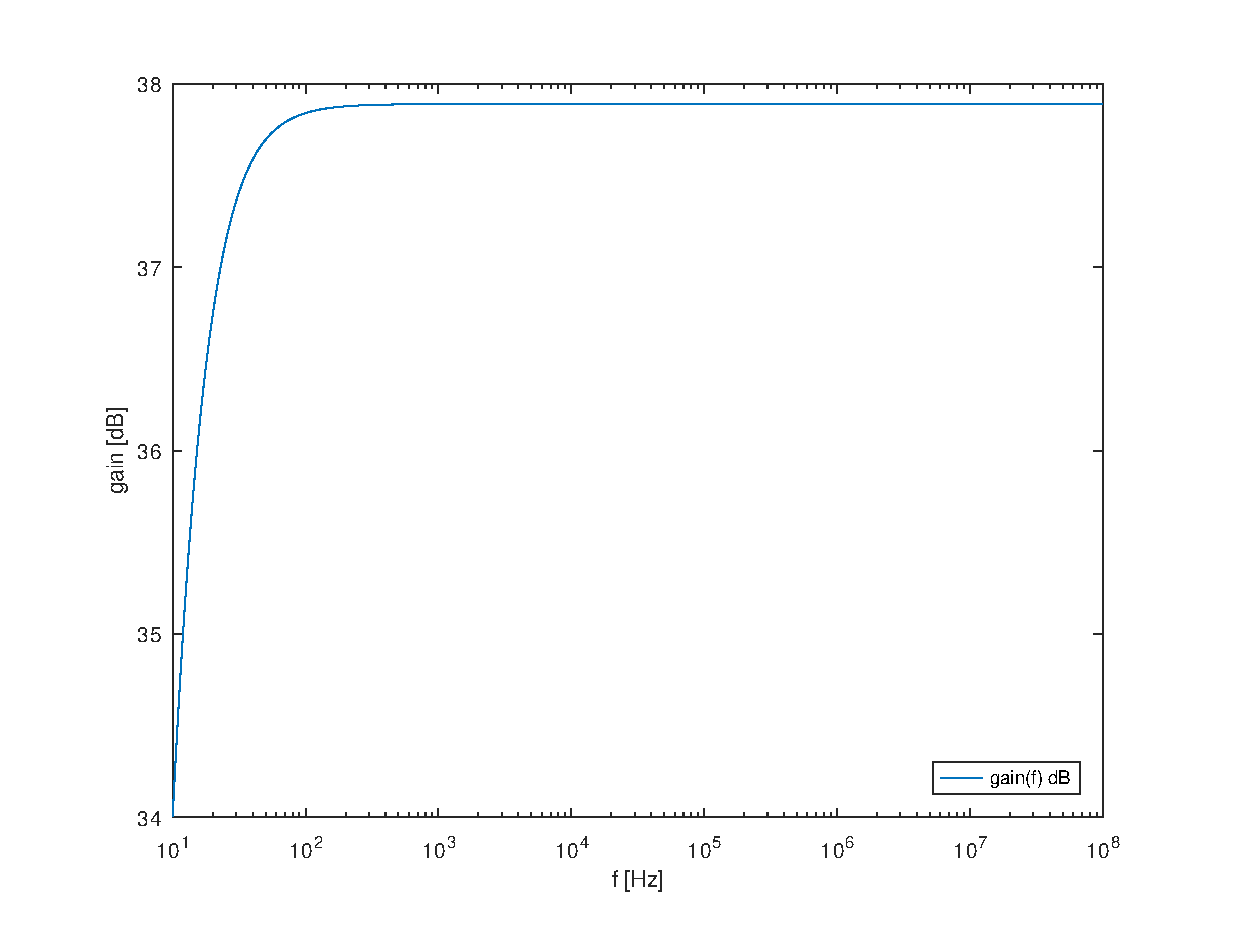
\includegraphics[width=0.6\linewidth]{gain_db_teo.eps}
\caption{Output voltage gain in order to frequency}
\label{fig:gain}
\end{figure}
\FloatBarrier

Here we present the merit figure of our circuit.

\begin{table}[h]
  \centering
  \begin{tabular}{|l|r|}
    \hline    
    {\bf Name} & {\bf Value [Mu]} \\ \hline
    $cost$ & 8116.008\\ \hline
$merit$ & 3492.661\\ \hline

  \end{tabular}
  \caption{Merit figure}
  \label{tab:OP}
\end{table}
\FloatBarrier
